\chapter{Filtre}
\section{Introduction}
Le MLI a besoin d'un signal sinusoïdal pour fonctionner, cependant, le VCO fournit un
signal triangulaire. Il est donc nécessaire d'avoir un filtre intermédiaire permettant
de transformer le signal de sortie du VCO en signal sinusoïdal ou tout du moins pseudo-sinusoïdal.
L'objectif de ce filtre est donc d'obtenir un graphe d'entrée-sortie similaire à
celui présenté sur la figure \ref{fig:filter-in-out}.

% TODO : refaire ce graphe avec les bon titres
\begin{figure}[ht]
	\centering
	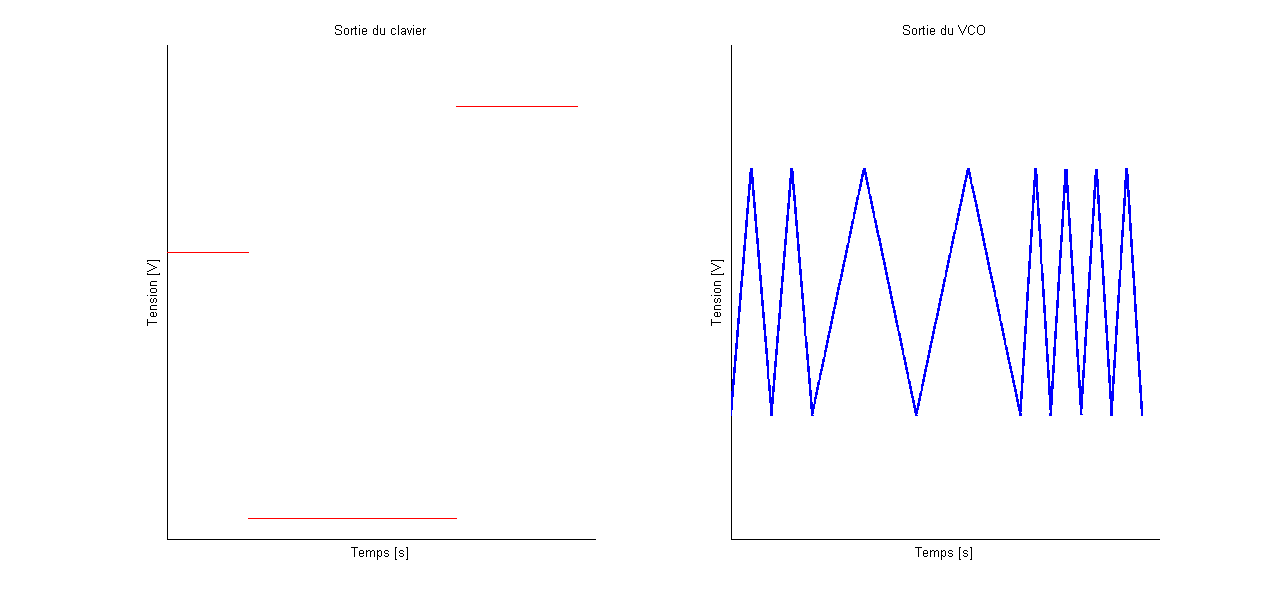
\includegraphics[scale=0.4]{img-filter/in-out.png}
	\caption{Entrée et sortie du filtre : objectif.}
	\label{fig:filter-in-out}
\end{figure}

\section{Fonctionnement}

\begin{figure}[ht]
	\centering
	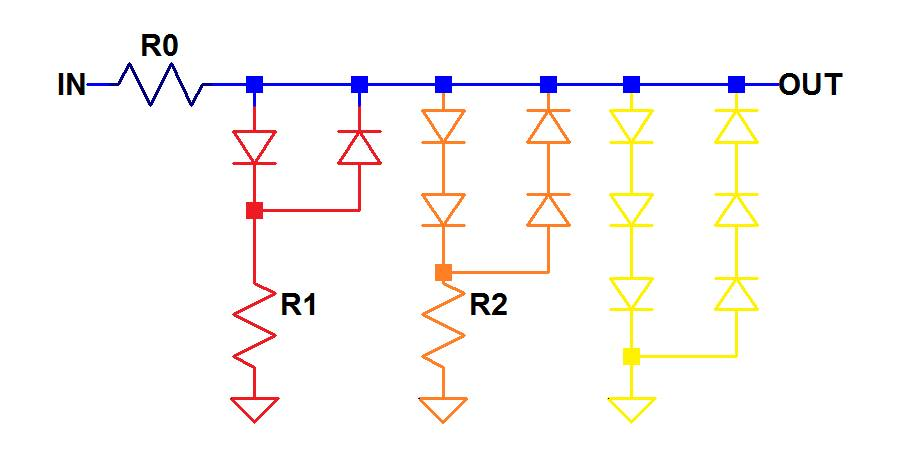
\includegraphics[scale=0.3]{img-filter/circuit-colored.png}
	\caption{Circuit du filtre.}
	\label{fig:circuit-filtre}
\end{figure}

Le filtre utilise des diodes pour faire varier le circuit en fonction de la tension d'entrée. 
Le circuit possède ainsi 4 états différents selon sa tension d'entrée :
\begin{enumerate}
	\item Elle est trop basse pour traverser la moindre diode :\\
				Dans ce cas-ci, seule la partie bleue du circuit est active, 
				il n'y a pas de courant, la tension d'entrée est don égale à
				la tension de sortie ;
	\item Elle est suffisante pour traverse une diode :\\
				Ici, la partie rouge du circuit (voir figure \ref{fig:circuit-filtre} est active. 
				On se retrouve donc avec un diviseur de tension qui diminuera la tension de sortie par rapport à la valeur d'entrée ;
	\item Elle est suffisante pour traverser deux diodes :\\
				La partie orange s'active en plus, ce qui mettra en parallèle les resistances $R_1$ et $R_2$ et
				réduira donc encore d'avantage la tension de sortie ;
	\item Elle est suffisante pour être écrêter par trois diodes :\\
				À partir d'ici, la résistance interne des 3 diodes jaunes va se mettre en parallèle avec $R_1$ et $R_2$
				\footnote{Si les diodes étaient idéales,
				le circuit fonctionnerait moins bien : au lieu d'obtenir un sommet de courbe de tension 
				arrondi dû à la résistance dynamique des diodes, on aurait un sommet de courbe
				horizontal à cause du lien direct à la masse. On pourrait cependant rajouter une résistance
				$R_3$ très faible derière les diodes pour redresser légèrement le sommet de la courbe.}. Étant donné que la 
				resistance interne des diodes est très faible comparée à $R_0$, il n'y a que peu de tension
				qui s'ajoutera encore à la tension de sortie.
\end{enumerate}

\section{Détails du circuit}

\begin{enumerate}
	\item Signal d'entrée :\\
				Le signal d'entrée doit être suffisament grand pour commencer à être
				écrêter par trois diodes en série, le signal de sortie culminera donc
				aux alentours de \unit{1.9}{\volt}. Le signal d'entrée est donc le signal
				triangulaire circonscrit au signal sinusoïdal d'amplitude \unit{1.9}{\volt},
				soit un signal triangulaire d'amplitude \unit{3}{\volt} ;
	\item Valeur des résistances : \\
		\begin{enumerate}
			\item Première approximation : $R_0$ a été définie à \unit{1}{\kilo\ohm}. $R_1$ quant à lui
						a été défini à \unit{7.9}{\kilo\ohm} afin que la pente de la tension avec 
						le diviseur $R_0$/$R_1$ soit égale à la pente moyenne de $y = 1.9\sin{Cx}$ entre $y=0.6$
						et $y = 1.2$ (soit $0.87C$). $R_2$ vaut \unit{2.2}{\kilo\ohm} afin que la pente de la 
						tension avec le diviseur $R_0$/($R_1$//$R_2$) soit égale à la pente moyenne de $y = 1.9\sin{Cx}$
						entre $y = 1.2$ et $y = 1.8$ (soit $0.58C$)

						Avec cette première approximation, le taux de distortion harmonique total est compris entre 0.51\% 
						(\unit{500}{\hertz}) et 0.5\%(\unit{10}{\kilo\hertz}).
						% FIX : compris entre 0.51 et 0.5, really ?!?
			\item Seconde approximation : pour améliorer ensuite le pseudo-sinus, des tests empiriques ont amené
						à une valeur de \unit{12.1}{\kilo\ohm} pour $R_1$ et de \unit{2.1}{\kilo\ohm} pour $R_2$.\\
						Avec ces nouvelles valeurs, le taux de distortion harmonique total est compris entre 0.3\% 
						(\unit{500}{\hertz}) et 0.23\% (\unit{10}{\kilo\hertz}). Les FFT
						théoriques (réalisées avec LTSpice) du signal d'entrée, du signal de sortie et d'un sinusoïdale
						pure sont présentées sur la figure \ref{fig:fft-filtre}.
		\end{enumerate}
\end{enumerate}

\begin{figure}[ht]
	\centering
	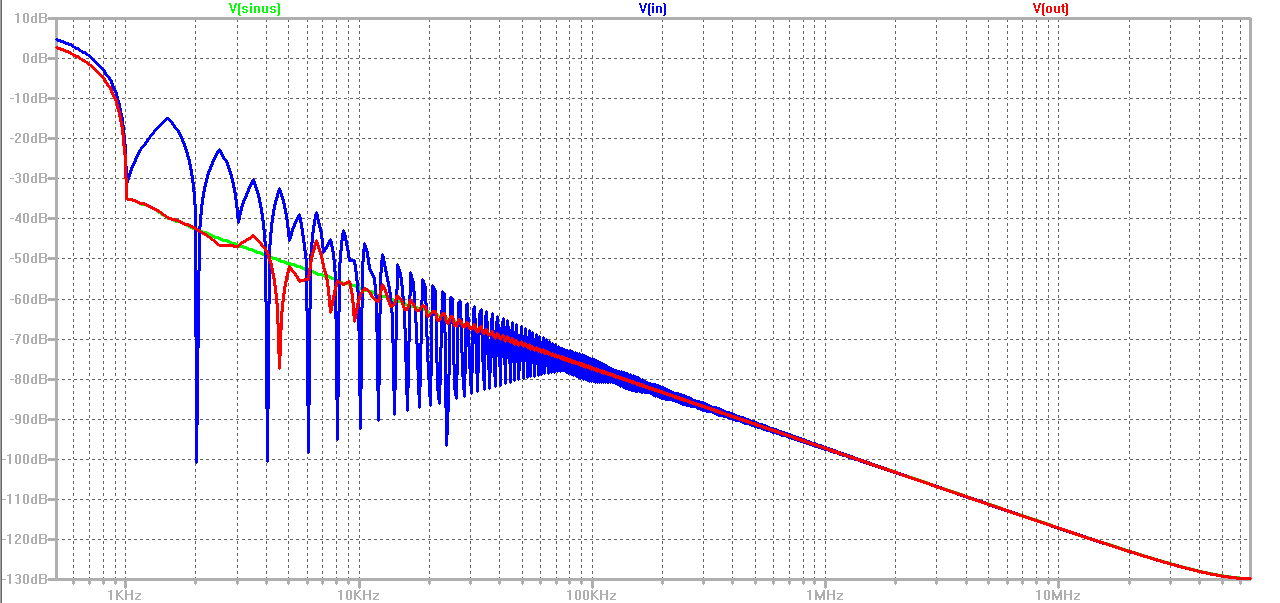
\includegraphics[scale=0.3]{img-filter/FFT.png}
	\caption{FFT avec les résistances de la seconde estimation.}
	\label{fig:fft-filtre}
\end{figure}

\section{Confontation théorie et mesures}

\begin{figure}[ht]
	\centering
	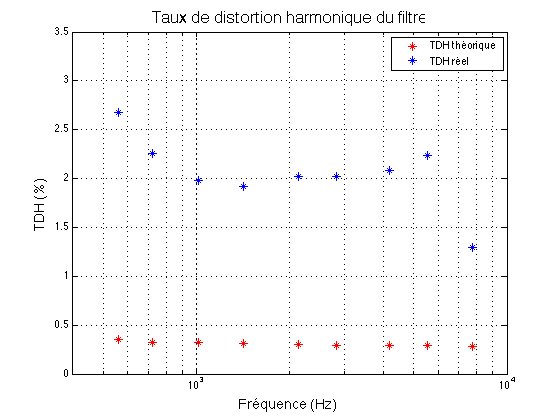
\includegraphics[scale=0.3]{img-filter/THD.png}
	\caption{Confrontation THD réel et théorique}
	\label{fig:thd-filtre}
\end{figure}

Dans la pratique, le TDH\footnote{Pour taux de distortion harmonique} 
est non seulement beaucoup plus important que dans la réalité, mais aussi beaucoup plus 
variable (voir figure \ref{fig:thd-filtre}). Cela est principalement dû au manque de précision des composants dans le filtre
et en amont\footnote{En effet, cela cause une imprécision dans le signal d'entrée du filtre
qui n'est pas exactement un signal triangulaire \unit{+3}{\volt}/\unit{-3}{\volt}}. Mais c'est
aussi dû aux glitchs provoqués par le MLI qui perturbent le pseudo-sinus.

\section{Améliorations possibles}

\begin{enumerate}
	\item Coder un programme capable de calculer avec précision $R_0$, $R_1$, $R_2$ et la tension 
				d'entrée afin de réduire au maximum le taux de distortion harmonique ;
	\item S'arranger pour que les données pratiques soient plus proches des données théoriques afin 
				de minimiser l'erreur dûe à la tolérance des composants.
\end{enumerate}